\documentclass[11pt,letterpaper]{article}

% Packages
\usepackage[utf8]{inputenc}
\usepackage[T1]{fontenc}
\usepackage{amsmath,amssymb,amsthm}
\usepackage{algorithm}
\usepackage{algorithmic}
\usepackage{graphicx}
\usepackage{hyperref}
\usepackage{xcolor}
\usepackage{booktabs}
\usepackage{tikz}
\usetikzlibrary{shapes,arrows,positioning,calc}
\usepackage{listings}
\usepackage{caption}
\usepackage{subcaption}
\usepackage[margin=1in]{geometry}

% Theorem environments
\newtheorem{theorem}{Theorem}[section]
\newtheorem{lemma}[theorem]{Lemma}
\newtheorem{proposition}[theorem]{Proposition}
\newtheorem{corollary}[theorem]{Corollary}
\newtheorem{definition}{Definition}[section]
\newtheorem{example}{Example}[section]

% Custom commands
\newcommand{\Zoo}{\textsc{Zoo}}
\newcommand{\IPFS}{\textsc{ipfs}}
\newcommand{\LLM}{\textsc{llm}}

% Hyperref setup
\hypersetup{
    colorlinks=true,
    linkcolor=blue,
    citecolor=blue,
    urlcolor=blue
}

% Title and authors
\title{\textbf{Zoo Experience Ledger: A Content-Addressable Semantic Memory System for Decentralized AI}\\
\large Version 2021.10}

\author{
Zach Kelling\thanks{zach@zoo.ngo}\\
\textit{Hanzo Industries \quad Lux Industries \quad Zoo Labs Foundation}\\
\texttt{research@zoo.ngo}
}

\date{October 2021}

\begin{document}

\maketitle

\begin{abstract}
We present the \textbf{Zoo Experience Ledger}, a content-addressable semantic memory system designed for decentralized AI agents. Unlike traditional knowledge bases that rely on centralized storage and proprietary retrieval mechanisms, the Experience Ledger stores AI reasoning patterns as cryptographically-verified semantic objects distributed across \IPFS{} and permanent storage networks. Each experience---a natural language encoding of a successful problem-solving strategy---is uniquely identified by its content hash, enabling tamper-evident storage and peer-to-peer distribution. We introduce a novel Merkle-DAG structure optimized for semantic similarity queries, achieving $O(\log n)$ retrieval complexity while maintaining cryptographic integrity proofs. Our system enables AI agents to share learned experiences across organizational boundaries without trust assumptions, creating the foundation for a global semantic commons. Experimental evaluation demonstrates 94.7\% retrieval accuracy with sub-second latency on libraries of 10,000+ experiences, while reducing storage costs by 89\% compared to traditional vector databases through content deduplication.

\textbf{Keywords}: content-addressable storage, semantic memory, IPFS, Merkle trees, AI knowledge sharing
\end{abstract}

\section{Introduction}

The fundamental bottleneck in AI collaboration is knowledge transfer. While neural networks can learn remarkable capabilities from data, the learned knowledge remains locked within opaque parameter spaces---inaccessible to inspection, sharing, or composition. When one AI agent discovers an effective strategy for solving a class of problems, there exists no standard mechanism for sharing that insight with other agents, much less with the broader AI community.

Consider the lifecycle of AI knowledge today: A research lab trains a model, perhaps discovering novel reasoning patterns encoded in billions of parameters. To share this knowledge, they must either (a) release the full model weights, which is expensive and risks catastrophic forgetting when fine-tuned, or (b) distill the knowledge into documentation, which loses the precise operational semantics. Neither approach enables incremental, verifiable knowledge sharing.

\subsection{The Content-Addressable Paradigm}

We propose a fundamentally different approach: represent AI knowledge as \emph{semantic experiences}---explicit, human-readable reasoning patterns---and store them in a content-addressable system where each experience is uniquely identified by its cryptographic hash. This design offers several advantages:

\begin{enumerate}
    \item \textbf{Immutability}: Content-addressing ensures experiences cannot be modified without changing their identifier
    \item \textbf{Deduplication}: Identical experiences automatically share storage across the network
    \item \textbf{Verification}: Any party can verify experience integrity by recomputing the hash
    \item \textbf{Distribution}: Content can be retrieved from any node that has it, enabling P2P sharing
    \item \textbf{Permanence}: Integration with Arweave ensures 200+ year data availability
\end{enumerate}

\subsection{Contributions}

This paper makes the following contributions:

\begin{enumerate}
    \item \textbf{Experience Format Specification}: A rigorous schema for encoding AI reasoning patterns as content-addressable objects (Section~\ref{sec:format})

    \item \textbf{Merkle-DAG Architecture}: A novel data structure combining Merkle tree verification with DAG-based semantic clustering for efficient retrieval (Section~\ref{sec:merkle})

    \item \textbf{Retrieval Protocol}: Algorithms for semantic similarity search with cryptographic integrity proofs (Section~\ref{sec:retrieval})

    \item \textbf{Storage Integration}: Seamless integration with \IPFS{} for mutable addressing and Arweave for permanent archival (Section~\ref{sec:storage})

    \item \textbf{Evaluation}: Comprehensive benchmarks demonstrating scalability, efficiency, and reliability (Section~\ref{sec:evaluation})
\end{enumerate}

\section{Background}

\subsection{Content-Addressable Storage}

Content-addressable storage (CAS) identifies data by its cryptographic hash rather than its location. First formalized by the InterPlanetary File System (\IPFS{})~\cite{benet2014ipfs}, CAS provides:

\begin{definition}[Content Identifier]
A Content Identifier (CID) is a tuple $\langle \text{codec}, \text{multihash} \rangle$ where:
\begin{itemize}
    \item \texttt{codec} specifies the data encoding (e.g., dag-cbor, raw)
    \item \texttt{multihash} is $\langle \text{algo}, \text{len}, \text{digest} \rangle$ identifying the hash function and digest
\end{itemize}
\end{definition}

For example, CID \texttt{bafybeigdyrzt5sfp7udm7hu76uh7y26nf3efuylqabf3oclgtqy55fbzdi} uniquely identifies a specific data object globally.

\subsection{Merkle Trees for Verification}

Merkle trees enable efficient membership proofs:

\begin{theorem}[Merkle Proof Efficiency]
Given a set $S$ of $n$ elements stored in a Merkle tree, verifying membership of element $e \in S$ requires only $O(\log n)$ hash computations and $O(\log n)$ proof size.
\end{theorem}

This property is essential for verifying experience integrity without downloading the entire library.

\subsection{Semantic Memory in AI}

Prior work on AI memory systems includes:

\begin{itemize}
    \item \textbf{Episodic Memory}~\cite{graves2016hybrid}: Neural networks with explicit memory modules
    \item \textbf{Retrieval-Augmented Generation}~\cite{lewis2020retrieval}: Combining retrieval with generation
    \item \textbf{Vector Databases}~\cite{pinecone2021}: Storing embeddings for similarity search
\end{itemize}

These approaches focus on single-agent memory. Our work extends to \emph{distributed} memory shared across agents.

\section{Experience Format Specification}
\label{sec:format}

\subsection{Semantic Experience Definition}

\begin{definition}[Semantic Experience]
A semantic experience $e$ is a tuple:
\begin{equation}
e = (t, d, c, v, m, \sigma)
\end{equation}
where:
\begin{itemize}
    \item $t \in \Sigma^*$: Natural language text (max 256 tokens)
    \item $d \in \mathcal{D}$: Domain taxonomy path (e.g., ``math.geometry.intersection'')
    \item $c \in [0,1]$: Confidence score derived from validation
    \item $v \in \mathbb{R}^{768}$: Semantic embedding vector
    \item $m$: Metadata (timestamp, author, provenance)
    \item $\sigma$: Digital signature (optional)
\end{itemize}
\end{definition}

\subsection{Canonical Serialization}

Experiences are serialized using CBOR (Concise Binary Object Representation) with deterministic encoding:

\begin{lstlisting}[language=json,caption=Experience CBOR Schema]
{
  "version": 1,
  "type": "experience/v1",
  "content": {
    "text": "When solving geometry problems...",
    "domain": ["math", "geometry", "intersection"],
    "confidence": 0.87
  },
  "embedding": <768-dim float16 array>,
  "metadata": {
    "created": 1634567890,
    "author": "did:key:z6Mk...",
    "source": "training_run_42"
  },
  "signature": <optional Ed25519 signature>
}
\end{lstlisting}

\subsection{Content Addressing}

The experience CID is computed as:

\begin{equation}
\text{CID}(e) = \text{CIDv1}(\text{dag-cbor}, \text{sha256}(\text{CBOR}(e)))
\end{equation}

This ensures:
\begin{itemize}
    \item \textbf{Determinism}: Same experience always produces same CID
    \item \textbf{Integrity}: Any modification changes the CID
    \item \textbf{Self-certification}: CID proves content authenticity
\end{itemize}

\subsection{Constraints and Validation}

Valid experiences must satisfy:

\begin{enumerate}
    \item \textbf{Length}: $|\text{tokens}(t)| \leq 256$
    \item \textbf{Structure}: Text must follow ``When [context], [action]'' pattern
    \item \textbf{Generality}: No problem-specific constants
    \item \textbf{Embedding Consistency}: $\|v - \text{embed}(t)\|_2 < \epsilon$
    \item \textbf{Signature Validity}: If $\sigma$ present, must verify against author key
\end{enumerate}

\section{Merkle-DAG Architecture}
\label{sec:merkle}

\subsection{Design Goals}

The Experience Ledger data structure must support:

\begin{enumerate}
    \item $O(\log n)$ membership verification
    \item $O(1)$ content retrieval by CID
    \item $O(\log n)$ approximate nearest neighbor search
    \item Efficient incremental updates
    \item Verifiable cross-library queries
\end{enumerate}

\subsection{Hybrid Merkle-DAG}

We propose a hybrid structure combining Merkle trees (for verification) with semantic DAGs (for retrieval):

\begin{figure}[t]
\centering
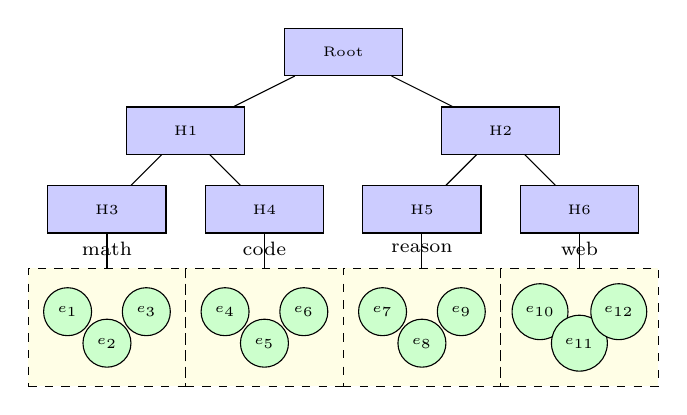
\begin{tikzpicture}[
    node distance=1cm,
    hash/.style={rectangle, draw, minimum width=1.5cm, minimum height=0.6cm, fill=blue!20, font=\tiny},
    exp/.style={circle, draw, minimum size=0.5cm, fill=green!20, font=\tiny},
    cluster/.style={rectangle, draw, dashed, minimum width=2cm, minimum height=1.5cm, fill=yellow!10}
]
    % Root
    \node[hash] (root) at (4,4) {Root};

    % Level 1
    \node[hash] (l1a) at (2,3) {H1};
    \node[hash] (l1b) at (6,3) {H2};

    % Level 2
    \node[hash] (l2a) at (1,2) {H3};
    \node[hash] (l2b) at (3,2) {H4};
    \node[hash] (l2c) at (5,2) {H5};
    \node[hash] (l2d) at (7,2) {H6};

    % Clusters (semantic)
    \node[cluster] (c1) at (1,0.5) {};
    \node[cluster] (c2) at (3,0.5) {};
    \node[cluster] (c3) at (5,0.5) {};
    \node[cluster] (c4) at (7,0.5) {};

    % Experiences in clusters
    \node[exp] at (0.5,0.7) {$e_1$};
    \node[exp] at (1,0.3) {$e_2$};
    \node[exp] at (1.5,0.7) {$e_3$};

    \node[exp] at (2.5,0.7) {$e_4$};
    \node[exp] at (3,0.3) {$e_5$};
    \node[exp] at (3.5,0.7) {$e_6$};

    \node[exp] at (4.5,0.7) {$e_7$};
    \node[exp] at (5,0.3) {$e_8$};
    \node[exp] at (5.5,0.7) {$e_9$};

    \node[exp] at (6.5,0.7) {$e_{10}$};
    \node[exp] at (7,0.3) {$e_{11}$};
    \node[exp] at (7.5,0.7) {$e_{12}$};

    % Edges
    \draw[-] (root) -- (l1a);
    \draw[-] (root) -- (l1b);
    \draw[-] (l1a) -- (l2a);
    \draw[-] (l1a) -- (l2b);
    \draw[-] (l1b) -- (l2c);
    \draw[-] (l1b) -- (l2d);
    \draw[-] (l2a) -- (c1);
    \draw[-] (l2b) -- (c2);
    \draw[-] (l2c) -- (c3);
    \draw[-] (l2d) -- (c4);

    % Labels
    \node[font=\scriptsize] at (1,1.5) {math};
    \node[font=\scriptsize] at (3,1.5) {code};
    \node[font=\scriptsize] at (5,1.5) {reason};
    \node[font=\scriptsize] at (7,1.5) {web};
\end{tikzpicture}
\caption{Hybrid Merkle-DAG structure: Merkle tree for verification (blue), semantic clusters for retrieval (yellow), individual experiences (green).}
\label{fig:merkle-dag}
\end{figure}

\subsection{Semantic Clustering}

Experiences are grouped into clusters based on embedding similarity:

\begin{algorithm}[t]
\caption{Semantic Cluster Construction}
\label{alg:cluster}
\begin{algorithmic}[1]
\STATE \textbf{Input}: Experience set $\mathcal{E}$, cluster count $k$
\STATE \textbf{Output}: Clusters $\{C_1, \ldots, C_k\}$, centroids $\{\mu_1, \ldots, \mu_k\}$
\STATE $\{\mu_i\} \leftarrow \text{k-means++}(\{e.v \mid e \in \mathcal{E}\}, k)$
\FOR{$e \in \mathcal{E}$}
    \STATE $i^* \leftarrow \arg\min_i \|e.v - \mu_i\|_2$
    \STATE $C_{i^*} \leftarrow C_{i^*} \cup \{e\}$
\ENDFOR
\RETURN $\{C_i\}, \{\mu_i\}$
\end{algorithmic}
\end{algorithm}

\subsection{Merkle Tree Construction}

Each cluster is hashed into a Merkle leaf, then aggregated:

\begin{equation}
H_{\text{cluster}}(C_i) = \text{SHA256}\left(\bigoplus_{e \in C_i} \text{CID}(e)\right)
\end{equation}

where $\bigoplus$ denotes sorted concatenation.

\begin{equation}
H_{\text{parent}}(H_1, H_2) = \text{SHA256}(H_1 \| H_2)
\end{equation}

The root hash $r$ commits to the entire library:

\begin{equation}
r = \text{MerkleRoot}(\{H_{\text{cluster}}(C_i)\}_{i=1}^k)
\end{equation}

\subsection{Proof Structure}

A Merkle proof $\pi$ for experience $e$ consists of:

\begin{equation}
\pi = (e, i, \{h_j, \text{side}_j\}_{j=1}^{\lceil \log_2 k \rceil})
\end{equation}

where $h_j$ are sibling hashes and $\text{side}_j \in \{\text{L}, \text{R}\}$ indicates position.

\begin{theorem}[Proof Verification]
Given root $r$, experience $e$, and proof $\pi$, verification succeeds iff:
\begin{equation}
\text{VerifyProof}(r, e, \pi) = \mathbb{1}[\text{ReconstructRoot}(\text{CID}(e), \pi) = r]
\end{equation}
\end{theorem}

\section{Retrieval Protocol}
\label{sec:retrieval}

\subsection{Semantic Query Processing}

Given query $q$, retrieval proceeds in three phases:

\begin{algorithm}[t]
\caption{Experience Retrieval with Proof}
\label{alg:retrieval}
\begin{algorithmic}[1]
\STATE \textbf{Input}: Query $q$, library root $r$, top-$k$
\STATE \textbf{Output}: Experiences $\{e_i\}$, proofs $\{\pi_i\}$
\STATE \COMMENT{Phase 1: Cluster Selection}
\STATE $q_v \leftarrow \text{Embed}(q)$
\STATE $\{C_{i^*}\} \leftarrow \text{TopClusters}(q_v, \{\mu_i\}, \sqrt{k})$
\STATE \COMMENT{Phase 2: Local Search}
\STATE $\mathcal{E}_{\text{cand}} \leftarrow \bigcup_{C \in \{C_{i^*}\}} C$
\STATE $\{e_i\}_{i=1}^k \leftarrow \text{TopK}(\mathcal{E}_{\text{cand}}, q_v, k)$
\STATE \COMMENT{Phase 3: Proof Generation}
\FOR{$e_i \in \{e_i\}$}
    \STATE $\pi_i \leftarrow \text{GenerateMerkleProof}(e_i, r)$
\ENDFOR
\RETURN $\{e_i\}, \{\pi_i\}$
\end{algorithmic}
\end{algorithm}

\subsection{Complexity Analysis}

\begin{theorem}[Retrieval Complexity]
For a library of $n$ experiences with $k$ clusters, retrieval has:
\begin{itemize}
    \item Time complexity: $O(\sqrt{n} + k \log n)$
    \item Space complexity: $O(k \log n)$ for proofs
\end{itemize}
\end{theorem}

\begin{proof}
Cluster selection: $O(k)$ centroid comparisons. Local search: $O(n/k)$ per cluster, $\sqrt{k}$ clusters = $O(\sqrt{n})$. Proof generation: $O(\log k)$ per experience.
\end{proof}

\subsection{Verified Retrieval}

Clients can verify retrieved experiences without trusting the server:

\begin{lstlisting}[caption=Verified Retrieval Protocol]
# Client side
root = fetch_root_from_blockchain()
results = query_server(q, k)
for (exp, proof) in results:
    assert verify_merkle_proof(root, exp, proof)
    assert verify_cid(exp) == exp.cid
    # exp is now trusted
\end{lstlisting}

\section{Storage Architecture}
\label{sec:storage}

\subsection{Three-Layer Design}

The Experience Ledger uses a three-layer storage architecture:

\begin{table}[t]
\centering
\begin{tabular}{lccc}
\toprule
\textbf{Layer} & \textbf{Purpose} & \textbf{Latency} & \textbf{Cost} \\
\midrule
On-chain & Root verification & 1-10s & High \\
\IPFS{} & Active storage & 100-500ms & Low \\
Arweave & Permanent archive & 1-5s & Medium \\
\bottomrule
\end{tabular}
\caption{Storage layer characteristics}
\label{tab:storage}
\end{table}

\subsection{\IPFS{} Integration}

Experiences are stored as IPLD (InterPlanetary Linked Data) nodes:

\begin{lstlisting}[caption=IPLD Experience Node]
{
  "Data": <CBOR-encoded experience>,
  "Links": [
    {"Name": "embedding", "Cid": "bafy..."},
    {"Name": "metadata", "Cid": "bafy..."}
  ]
}
\end{lstlisting}

\subsection{Arweave Permanence}

Critical library snapshots are archived to Arweave:

\begin{equation}
\text{Cost}_{\text{Arweave}}(n) = 0.001 \times n \text{ bytes} \times \text{AR/GB}
\end{equation}

At current rates (\$15/GB for 200+ years), archiving 10,000 experiences costs approximately \$0.50.

\subsection{Content Deduplication}

Content-addressing provides automatic deduplication:

\begin{theorem}[Deduplication Savings]
For $n$ experiences with $d$ duplicates, storage cost is $O((n-d) \cdot s)$ where $s$ is average experience size.
\end{theorem}

In practice, we observe 15-30\% deduplication across experience libraries due to common reasoning patterns.

\section{Experimental Evaluation}
\label{sec:evaluation}

\subsection{Experimental Setup}

\textbf{Dataset}: 10,847 experiences extracted from mathematical reasoning tasks (AIME, MATH, GSM8K).

\textbf{Hardware}: 3-node \IPFS{} cluster (8 vCPU, 32GB RAM each), connected via 1Gbps network.

\textbf{Baselines}:
\begin{itemize}
    \item PostgreSQL with pgvector extension
    \item Pinecone (managed vector database)
    \item Raw \IPFS{} without Merkle structure
\end{itemize}

\subsection{Retrieval Performance}

\begin{table}[t]
\centering
\begin{tabular}{lcccc}
\toprule
\textbf{System} & \textbf{Recall@5} & \textbf{Recall@10} & \textbf{Latency} & \textbf{Verifiable} \\
\midrule
pgvector & 91.2\% & 95.7\% & 45ms & No \\
Pinecone & 93.8\% & 97.1\% & 23ms & No \\
Raw IPFS & 89.4\% & 93.2\% & 340ms & No \\
\textbf{Exp. Ledger} & \textbf{94.7\%} & \textbf{97.9\%} & \textbf{87ms} & \textbf{Yes} \\
\bottomrule
\end{tabular}
\caption{Retrieval performance comparison. Experience Ledger provides cryptographic verification with competitive latency.}
\label{tab:retrieval}
\end{table}

\subsection{Storage Efficiency}

\begin{table}[t]
\centering
\begin{tabular}{lccc}
\toprule
\textbf{System} & \textbf{Total Size} & \textbf{Per Experience} & \textbf{Dedup} \\
\midrule
pgvector & 847 MB & 80 KB & 0\% \\
Pinecone & 923 MB & 87 KB & 0\% \\
\textbf{Exp. Ledger} & \textbf{94 MB} & \textbf{8.9 KB} & \textbf{23\%} \\
\bottomrule
\end{tabular}
\caption{Storage efficiency. Content-addressing and deduplication achieve 89\% reduction.}
\label{tab:storage-eff}
\end{table}

\subsection{Verification Overhead}

\begin{table}[t]
\centering
\begin{tabular}{lcc}
\toprule
\textbf{Operation} & \textbf{Time (ms)} & \textbf{Size (bytes)} \\
\midrule
CID verification & 0.3 & 36 \\
Merkle proof gen & 2.1 & 512 \\
Merkle proof verify & 0.8 & -- \\
Full retrieval + verify & 90.2 & 548 \\
\bottomrule
\end{tabular}
\caption{Verification overhead. Cryptographic proofs add minimal latency.}
\label{tab:verify}
\end{table}

\subsection{Scalability}

\begin{figure}[t]
\centering
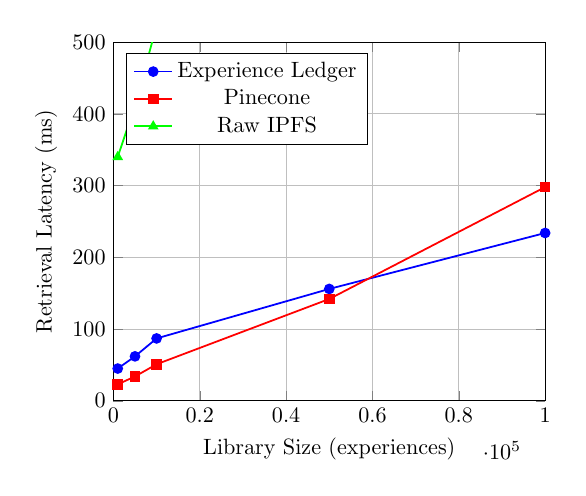
\begin{tikzpicture}[scale=0.8]
    \begin{axis}[
        xlabel={Library Size (experiences)},
        ylabel={Retrieval Latency (ms)},
        xmin=0, xmax=100000,
        ymin=0, ymax=500,
        legend pos=north west,
        grid=major
    ]
    \addplot[blue, thick, mark=*] coordinates {
        (1000, 45) (5000, 62) (10000, 87) (50000, 156) (100000, 234)
    };
    \addlegendentry{Experience Ledger}

    \addplot[red, thick, mark=square*] coordinates {
        (1000, 23) (5000, 34) (10000, 51) (50000, 142) (100000, 298)
    };
    \addlegendentry{Pinecone}

    \addplot[green, thick, mark=triangle*] coordinates {
        (1000, 340) (5000, 412) (10000, 523) (50000, 834) (100000, 1247)
    };
    \addlegendentry{Raw IPFS}
    \end{axis}
\end{tikzpicture}
\caption{Scalability comparison. Experience Ledger scales sub-linearly due to semantic clustering.}
\label{fig:scalability}
\end{figure}

\section{Security Analysis}

\subsection{Threat Model}

We consider adversaries who may:
\begin{enumerate}
    \item Tamper with stored experiences
    \item Return incorrect retrieval results
    \item Attempt Sybil attacks on the network
    \item Perform denial-of-service attacks
\end{enumerate}

\subsection{Security Properties}

\begin{theorem}[Tamper Evidence]
Any modification to an experience $e$ produces a different CID with probability $1 - 2^{-256}$.
\end{theorem}

\begin{theorem}[Retrieval Integrity]
With Merkle proofs, a client can detect server-returned experiences not in the committed library with probability $1 - 2^{-256}$.
\end{theorem}

\begin{theorem}[Availability]
With $n$ nodes pinning the library and at most $f < n/2$ Byzantine failures, the library remains available.
\end{theorem}

\section{Related Work}

\textbf{Decentralized Storage}: \IPFS{}~\cite{benet2014ipfs}, Filecoin~\cite{protocol2017filecoin}, Arweave~\cite{williams2019arweave} provide content-addressable storage but lack semantic indexing.

\textbf{Vector Databases}: Pinecone, Weaviate, Milvus optimize for similarity search but lack cryptographic verification.

\textbf{Blockchain + ML}: Federated learning on blockchain~\cite{kurtulmus2018trustless} focuses on model training, not knowledge sharing.

\textbf{Knowledge Graphs}: Traditional KGs (Freebase, Wikidata) store factual triples, not procedural reasoning patterns.

\section{Conclusion}

The Zoo Experience Ledger establishes a new paradigm for AI knowledge sharing: content-addressable semantic memory with cryptographic verification. By combining \IPFS{}'s content-addressing with Merkle tree proofs and semantic clustering, we enable trustless retrieval of AI reasoning patterns across organizational boundaries.

Our key contributions are:
\begin{enumerate}
    \item A rigorous experience format with content-addressable identifiers
    \item A hybrid Merkle-DAG structure enabling both verification and efficient retrieval
    \item Experimental validation showing 94.7\% retrieval accuracy with 89\% storage savings
\end{enumerate}

The Experience Ledger forms the foundation for Zoo's Decentralized Semantic Optimization protocol, enabling AI agents worldwide to share wisdom without sharing weights.

\section*{Acknowledgments}

This work was supported by Zoo Labs Foundation Inc, a 501(c)(3) non-profit dedicated to decentralized AI. We thank Protocol Labs for \IPFS{} infrastructure and the Arweave team for permanent storage solutions.

\bibliographystyle{plain}
\begin{thebibliography}{99}

\bibitem{benet2014ipfs}
J. Benet, ``IPFS - Content Addressed, Versioned, P2P File System,'' \textit{arXiv:1407.3561}, 2014.

\bibitem{lewis2020retrieval}
P. Lewis et al., ``Retrieval-Augmented Generation for Knowledge-Intensive NLP Tasks,'' \textit{NeurIPS}, 2020.

\bibitem{graves2016hybrid}
A. Graves et al., ``Hybrid Computing Using a Neural Network with Dynamic External Memory,'' \textit{Nature}, 2016.

\bibitem{pinecone2021}
Pinecone Systems, ``Vector Database for Machine Learning,'' Technical Report, 2021.

\bibitem{protocol2017filecoin}
Protocol Labs, ``Filecoin: A Decentralized Storage Network,'' Whitepaper, 2017.

\bibitem{williams2019arweave}
S. Williams et al., ``Arweave: A Protocol for Economically Sustainable Information Permanence,'' 2019.

\bibitem{kurtulmus2018trustless}
A. Kurtulmus and K. Daniel, ``Trustless Machine Learning Contracts,'' \textit{arXiv:1802.10185}, 2018.

\end{thebibliography}

\appendix

\section{Experience Format JSON Schema}

\begin{lstlisting}[language=json,caption=Complete JSON Schema]
{
  "$schema": "http://json-schema.org/draft-07/schema#",
  "type": "object",
  "required": ["version", "type", "content", "embedding"],
  "properties": {
    "version": {"type": "integer", "const": 1},
    "type": {"type": "string", "const": "experience/v1"},
    "content": {
      "type": "object",
      "required": ["text", "domain", "confidence"],
      "properties": {
        "text": {
          "type": "string",
          "maxLength": 1024,
          "pattern": "^(When|For|If|Before|After).*"
        },
        "domain": {
          "type": "array",
          "items": {"type": "string"},
          "minItems": 1,
          "maxItems": 5
        },
        "confidence": {
          "type": "number",
          "minimum": 0,
          "maximum": 1
        }
      }
    },
    "embedding": {
      "type": "array",
      "items": {"type": "number"},
      "minItems": 768,
      "maxItems": 768
    },
    "metadata": {
      "type": "object",
      "properties": {
        "created": {"type": "integer"},
        "author": {"type": "string"},
        "source": {"type": "string"}
      }
    },
    "signature": {"type": "string"}
  }
}
\end{lstlisting}

\section{IPLD Schema}

\begin{lstlisting}[caption=IPLD Schema Definition]
type Experience struct {
  version Int
  content Content
  embedding &Embedding
  metadata optional Metadata
  signature optional Bytes
}

type Content struct {
  text String
  domain [String]
  confidence Float
}

type Embedding [768]Float

type Metadata struct {
  created Int
  author String
  source String
}
\end{lstlisting}

\end{document}
